% !Rnw weave = knitr
\documentclass[12pt]{article}\usepackage[]{graphicx}\usepackage[]{color}
% maxwidth is the original width if it is less than linewidth
% otherwise use linewidth (to make sure the graphics do not exceed the margin)
\makeatletter
\def\maxwidth{ %
  \ifdim\Gin@nat@width>\linewidth
    \linewidth
  \else
    \Gin@nat@width
  \fi
}
\makeatother

\definecolor{fgcolor}{rgb}{0.345, 0.345, 0.345}
\newcommand{\hlnum}[1]{\textcolor[rgb]{0.686,0.059,0.569}{#1}}%
\newcommand{\hlstr}[1]{\textcolor[rgb]{0.192,0.494,0.8}{#1}}%
\newcommand{\hlcom}[1]{\textcolor[rgb]{0.678,0.584,0.686}{\textit{#1}}}%
\newcommand{\hlopt}[1]{\textcolor[rgb]{0,0,0}{#1}}%
\newcommand{\hlstd}[1]{\textcolor[rgb]{0.345,0.345,0.345}{#1}}%
\newcommand{\hlkwa}[1]{\textcolor[rgb]{0.161,0.373,0.58}{\textbf{#1}}}%
\newcommand{\hlkwb}[1]{\textcolor[rgb]{0.69,0.353,0.396}{#1}}%
\newcommand{\hlkwc}[1]{\textcolor[rgb]{0.333,0.667,0.333}{#1}}%
\newcommand{\hlkwd}[1]{\textcolor[rgb]{0.737,0.353,0.396}{\textbf{#1}}}%
\let\hlipl\hlkwb

\usepackage{framed}
\makeatletter
\newenvironment{kframe}{%
 \def\at@end@of@kframe{}%
 \ifinner\ifhmode%
  \def\at@end@of@kframe{\end{minipage}}%
  \begin{minipage}{\columnwidth}%
 \fi\fi%
 \def\FrameCommand##1{\hskip\@totalleftmargin \hskip-\fboxsep
 \colorbox{shadecolor}{##1}\hskip-\fboxsep
     % There is no \\@totalrightmargin, so:
     \hskip-\linewidth \hskip-\@totalleftmargin \hskip\columnwidth}%
 \MakeFramed {\advance\hsize-\width
   \@totalleftmargin\z@ \linewidth\hsize
   \@setminipage}}%
 {\par\unskip\endMakeFramed%
 \at@end@of@kframe}
\makeatother

\definecolor{shadecolor}{rgb}{.97, .97, .97}
\definecolor{messagecolor}{rgb}{0, 0, 0}
\definecolor{warningcolor}{rgb}{1, 0, 1}
\definecolor{errorcolor}{rgb}{1, 0, 0}
\newenvironment{knitrout}{}{} % an empty environment to be redefined in TeX

\usepackage{alltt}
\usepackage[backend=biber, sorting=nyt, maxcitenames=2, doi=false,url=false, style=apa]{biblatex} %add annotation=true and style=reading to print the annotations in the bibliography
\usepackage[american]{babel}
%\usepackage{newtxtext,newtxmath}
\usepackage{csquotes}
\bibliography{/home/harold/Dropbox/full,/home/harold/github/eysterthesis/manuscript/thesis_ref}
\DeclareLanguageMapping{american}{american-apa}
\usepackage[compact]{titlesec}
\usepackage{csquotes}
\usepackage{amsmath}
%\usepackage[hyphens]{url}
\usepackage[margin=1in]{geometry}
\usepackage{mathtools}
\setlength{\parskip}{.6em}
\usepackage{setspace}
\usepackage{multicol}
\usepackage{longtable}
\usepackage{makecell}
\renewcommand\theadalign{bc}
\renewcommand\theadfont{\bfseries}
\renewcommand\theadgape{\Gape[4pt]}
\renewcommand\cellgape{\Gape[4pt]}
\renewcommand{\tablename}{Table}
%\usepackage{sectsty}
%\allsectionsfont{\singlespacing}
%\usepackage{indentfirst} %This indents the pfaragraph following a heading 
\setlength{\parindent}{0em}
\usepackage{breqn}
\usepackage{xr}
\externaldocument{SI}
\usepackage{graphicx}
\usepackage{pdfpages}
\usepackage{subcaption}
\usepackage[figuresleft]{rotating}
\graphicspath{{home/harold/github/eysterthesis/manuscript/}} %make sure to include the slash after the colon at at the end 
%Make sure Bibliography --> is set as biblatex 
%Then run tools-->bibliography, then compile 
\usepackage{authblk}
\title{Invader success and changing climate: Comparisons in the native and introduced range of seven plant species}
\author[1]{Harold N. Eyster}
\author[2]{Elizabeth Wolkovich}
\affil[1]{Institute for Resources, Environment, and Sustainability, University of British Columbia}
\affil[2]{Department of Forest and Conservation Science, University of British Columbia}
\date{}                     %% if you don't need date to appear
\setcounter{Maxaffil}{0}
\renewcommand\Affilfont{\itshape\small}
\usepackage[export]{adjustbox}






\IfFileExists{upquote.sty}{\usepackage{upquote}}{}
\begin{document}
\maketitle
%	\fbox{\includegraphics[width=1 \textwidth,trim=0cm 0cm 0cm 0cm, clip=true]{comps_overview}}

\begin{spacing}{1} %1.9
	\begin{abstract} 
Invasive plants often have large impacts on ecosystems. Yet we lack a clear understanding of how some species become successful invaders while others do not. Two competing mechanisms have been posited: 1) post-introduction rapid evolution or 2) broad environmental tolerance in the source population. 
Discovering the determinants of invasion success requires more information on how these two mechanisms drive essential invasion traits, including germination rate, germination timing, and growth rate. 
Here, we tested for evidence of evolution in these traits by using growth chambers to provide common environments for seven herbaceous plant species sampled from multiple populations in their native (European) and invasive (North American) ranges. Chambers provided two levels of stratification---to simulate different winter lengths---and four temperature levels post-stratification---to simulate different spring conditions. Bayesian multilevel models enabled us to examine responses for each species, as well as across the suite of all seven species.
We found consistent results across all species: traits were largely insensitive to population origin, except in response to particular combinations of high-temperature and stratification, generally representing cold winters and warm springs. This suggests that germination and growth traits of exotic species need not evolve during invasions. Instead, our results suggest that broad environmental tolerance underlies invasion success for this suite of common invaders. 
	\end{abstract}
\end{spacing}		
	\section{Introduction} 
	%EMW24Apr: First paragraph seemed to leave reader hanging a little long as to what the two mechanisms were. Many ways to fix this I expect, I did one way below.  
	Exotic plant invasions  can transform biodiversity and ecosystems \parencite{Bellard2016, Pejchar2009,Mack2000}.%, and ecosystem function, services, and resilience \parencite{Bellard2016,Clavero2005,Walker1997,Daehler1999,Ehrenfeld2003,Wilcove1998,Pejchar2009,Pimentel2005,Pysek2010,OTA1993,Mack2000,Levine2003}.
	 Understanding the underlying drivers of invasions is important because invasions may be increasing: globalization is facilitating extra-range plant dispersal \parencite{Helmus2014}, and human alteration of ecosystems may provide new niche space \parencite{Tilman2001, Blois2013,Inouye2008,Harte2015}. Upon dispersing to a new environment, invasive species can thrive by filling vacant niches \parencite{Elton1958} or outperforming native plants in high-resource and variable environments \parencite{Davis2001,Daehler2003}. Changing environments, especially with anthropogenic climate change, could select for species that can take advantage of the newly created temporal niches and resources through shifts in the timing of flowering, fruiting, and other life history events. \parencite{Franks2007}. 
	
	This understanding the drivers of invasions requires first identifying the biological mechanisms that plants may use to invade. Two contrasting mechanisms have been posited to give some plants the capacity to exploit invasible environments: 1) post-introduction rapid evolution and 2) broad environmental tolerance in the source population. 

	%To invade new The first factor for determining invasion potential is dispersal. To become invasive, a species first needs a dispersal mechanism to establish in a non-native habitat \parencite{Mark2001,Westphal2008}. Humans have played an important role in facilitating recent plant dispersals \parencite{McKinney1999,Pysek2002,Vitousek1996}, and with increased globalization the spread of species outside their respective native ranges will only increase \parencite{Helmus2014}. Once a species is introduced to a novel region, however, it must also be able to successfully disperse beyond the initial introduction location to be considered fully invasive. Thus species with greater dispersal ability may be more successful invaders.  Nonetheless, any intrinsic biological dispersal advantage can be wholly dominated by intentional introduction, e.g., for agricultural or ornamental purposes, or by accidental human-facilitated mechanisms, such as the transportation of invasive species within contaminated mulch or gravel \parencite{Wittenberg2001}. 	
	%Managing this onrush of invasive species requires understanding the mechanisms that give some plants the capacity to exploit invasible environments \parencite{Hulme2013}
	A large body of literature suggests that rapid adaptive evolution is a key driver of invasion success  \parencite[e.g.,][]{Reznick2001, Prentis2008,Colautti2015,Lee2002invasion,Clements2011}.  Rapid evolution can enable nonindigenous species to adapt to vacant niches and take advantage of variable and high-resource environments, for example by evolving greater competitive ability  when released from natural enemies \parencite{Blossey1995,Bossdorf2005} or by evolving adaptive plasticity \parencite{Richards2006}. % %EMW8Apr -- suggest you cut this next sentence. you can bring it up in discussion if critical ... Many genetic characteristics have been identified to enable invasion, including additive genetic variation, epistasis, hybridization, genomic rearrangements, etc. \parencite[Reviewed in][]{Lee2002invasion}, while genetic drift and bottlenecks likely stifle invasion capacity \parencite{Bock2015}. 
	
	There are many clear examples of rapid evolution abetting plant invasions. Genetic studies of two North American herbaceous goldenrods that invaded Europe, \textit{Solidago altissima} and \textit{S. gigantea} (Asteraceae), showed post-introduction genetic changes in flowering time in response to temperature, due to selection on source-population genetic variation and development of new mutations \parencite{Weber1998}. Similarly, the invasive \textit{Centaurea solstitialis} (Asteraceae) in California evolved larger size from standing variation in the founding population \parencite{Barker2017}. Also in California, a similar study found that genetic adaptation was driving adaptive phenotypic variation in flowering time between high-altitude and desert populations of \textit{Capsella bursa-pastoris} (Brassicaceae) \parencite{Linde2001}. Invasion may even produce evolution sufficient to establish reproductive isolation and trigger speciation, in as few as 13 generations \parencite{Hendry2000}. If rapid evolution is so central to invader success, then managers should treat invasives not as static, homogeneous species, but as constantly adapting populations \parencite{Lee2002invasion}. %EMW24Apr I still like this last sentence!
	
	Yet, despite the support for the importance of rapid evolution, a competing body of literature suggests that invaders need not evolve. Instead, broad environmental tolerance, plasticity and generalist adaptations to human-dominated environments (i.e., weediness) within the source population may give invaders sufficient advantages, obviating the necessity of rapid evolution \parencite{Richards2006,Schwartz1994,Bock2015,Rejmanek1996,Baker1965}. %This is an longstanding theory. In 1965, Baker suggested that there were stable characteristics that made some species invasive: r-selected, high growth rates, broad environmental tolerance, etc. 
	Studies have found contrasting results regarding whether weediness in the native range is the best predictor of invasiveness %.  weedy in their native range are likely to be invasive in novel environments: a study of 274 plant species native to North and South America but naturalized in France showed that the best determinant of invasiveness was weediness in the home range
	\parencite[e.g.,][]{Maillet2000}, or not \parencite{Perrins1992,Mack1996}. Seeking a unified answer, a meta-analysis of 117 studies found that invasive plants were associated with performance-related traits, and concluded that it may be possible to predict future invaders by those traits \parencite{VanKleunen2010}. However, this reasoning ignores the possibility (as argued by the rapid evolution theory) that these performance-related traits only evolve post-introduction. 
	
	One reason why the importance of rapid evolution remains contested is because few experimental designs allow unambiguous discrimination between the two claims. Neither observational datasets \parencite[e.g.,][]{Wolkovich2013} nor experimental common gardens \parencite{Conner2004,Vitasse2009} are sufficient to discriminate. And while genetic studies can identify the existence of rapid evolution, they do not demonstrate the prevalence of this invasion mechanism. Instead, reciprocal common garden experiments with native and invader populations can test these theories \parencite[e.g.,][]{Lamarque2015,Williams2008}. For example, a reciprocal common garden experiment of two invasive maple species (\textit{Acer}, Sapindaceae) demonstrated that rapid evolution was important for one species, but plasticity was important for the other \parencite{Lamarque2015}.  This and other studies show the promise of reciprocal common garden experiments for testing invasion mechanisms. However, despite their utility, they are quite rare and typically only include one or two species due to the immense effort required. Growth chamber experiments offer an attractive alternative: they are easier to control and execute, thereby enabling a larger number of species to be tested and compared simultaneously. Moreover, growth chambers can precisely vary the environments that plants experience and provide high-resolution assessment of small differences in trait responses. Testing such a multitude of species with growth chambers could help identify the mechanism(s) important for invasion success.  
	
	Another reason why these claims are contested may be because different mechanisms underlie different traits. Some traits, such as flowering time, may be under rapid selection \parencite{Weber1998}, while others may be broadly tolerant and stable. This is likely partly because some traits are known to evolve faster than others \parencite{Weiss-Lehman2017}. The importance of rapid evolution vs. broad environmental tolerance should thus be couched in specific traits, rather than overall effects. Thus,  understanding invasions requires understanding the mechanisms driving traits most essential for invasion.
	
	Germination and growth traits are some of the most important for granting invasive success \parencite{Sattin1997, Maillet2000}: invasive success requires the capacity to germinate in novel environments and grow rapidly enough to compete with native flora \parencite{Grime1988}. Therefore, germination rate, germination timing, and growth rate may represent key invasion traits. At least some of these traits appear to be sensitive to environmental differences \parencite{Leger2007}.  In particular they should respond strongly to two major germination cues: stratification length and post-stratification temperature \parencite{Finch2006}. In temperate ecosystems, a cold stratification simulates winter. A minimum period of winter must often pass before seeds can germinate to ensure that seeds do not germinate during a mid-winter warm period \parencite{Baskin1998,Popay1970,Wulff1994}. Winter length is a key niche variable \parencite{Harte2015} and may show substantial spatial variation, independent of other climate variables \parencite{Bonan2003}.  Once the necessary stratification length has been achieved, temperature can cue that it is the appropriate time for a seed to break dormancy. Temperature also plays an important role in controlling plant growth rate \parencite{Egli1980,Guilioni2003}. Across multiple species, testing how invasive and native population germination and growth traits respond to the environment---via stratification length and post-stratification temperature--could test if rapid evolution or broad environmental tolerance drives invasion. 

	Seeking this more general appraisal of the importance of rapid evolution and broad environmental tolerance of germination and growth traits in invasive plants, this paper reports on a growth chamber experiment of the native (Europe) and introduced (North America) ranges of seven highly invasive herbaceous plant species, many of which have been shown to be responsive to climate. We tested the degree to which rapid evolution has occurred since the species colonized North America from Europe.  This work follows a growing interest in invaders and phenology \parencite[e.g.,][]{Seabloom:2003mg,Wolkovich2014}. Our growth chamber experiment enabled us to test the degree to which phenologies in native and invasive populations differ in their response to climate.  Specifically, we measured how germination rate, time to germination, and growth rate of invasive (American) and native (European) conspecific populations responded to a full-factorial design of two stratification lengths and four post-stratification temperatures. If rapid evolution is of generalizable importance to invasive plants, we expect to find that seeds from the invading populations (North America) will respond very differently to temperature and stratification treatments than the indigenous populations (Europe) for all or nearly all species. 
	\section{Methods}
	\subsection{Study species}
	Following Richardson's definition of invasive species \parencite[][, see Supp. for details]{Richardson2000, Richardson2011}, seeds were collected from eight herbaceous species that originated in Europe but were recently introduced to the US, where they have spread and produced substantial populations \parencite{Uva1997}:\textit{ Alliaria petiolata}(ALLPET), \textit{Capsella bursa-pastoris} (CAPBUR), \textit{Chelidonium majus} (CHEMAJ), \textit{Dactylis glomerata} (DACGLO),  \textit{Plantago lanceolata} (PLALAN), \textit{P.  major} (PLAMAJ), \textit{Rumex crispus} (RUMCRI), and \textit{Taraxacum officinale} (TAROFF). \textit{A. petiolata} exhibited minimal germination, and so was removed from the analysis. These species represent a mix of perennials, biennials, and annuals. Many were intentionally introduced for medicinal or forage uses (for additional details, see Supp.).  All of these species have proven prodigious invaders in the US, with many impacting crop production and transforming ecosystems \parencite[e.g.,][]{Froese2003,Wolfe2008}. 

	Furthermore, those of our study species that are included in the Concord Phenology Dataset \parencite[ \textit{Capsella bursa-pastoris, Chelidonium majus, Plantago lanceolata}, and \textit{Rumex crispus},][]{Willis:2008bf}, are on average flowering 4.5 days earlier than they did in the 1800s (compared to less than a day earlier for all 372 species in the dataset). This suggest that these invasive species exhibit flexible phenologies---flexibility that may be key to their success. Although this paper focuses on a different set of phenologies, the flexible flowering phenology suggests that these species may also exhibit flexible germination or growth rate traits. If so, this work will be able to identify whether this flexibility is due to rapid evolution. Thus, these species offer apt subjects to test the importance of rapid evolution in invader germination and growth traits. 

	\subsection{Seed collection} 
	We collected mature seeds from native European populations and invasive North American populations from 2015-06-15 to 2015-09-05. European seeds came from 63 individuals across 13 sites in nine European countries: Austria, Denmark, France, Germany, Liechtenstein, The Netherlands, Norway, Slovenia, and Switzerland.  North American seeds came from 21 individuals across three sites  in Massachusetts, USA: Harvard Forest LTER (Petersham) Arnold Arboretum at Harvard University (Boston), and Walden Pond (Concord) (see \ref{fig:sites}). Elevation ranged from 0--1202 m in Europe and 20--300 m in USA. Seeds were collected in paper envelopes and stored at standard room temperature until early September 2015, when they were cleaned and returned to envelopes.  % For each plant we recorded: species, date, name of site, notes on human disturbance at site, abundance of the species at the site, aspect, elevation, GPS coordinates, height of the individual, spread of the individual, photo of the site, photo of at least one individual/site, and soil type.
	%\paragraph{European (native) seed collection} We collected European seeds from early-June to mid-July 2015 from 63 individuals across 13 sites in nine European countries: France, The Netherlands, Germany, Denmark, Norway, Austria, Slovenia, Liechtenstein, and Switzerland (see Figure \ref{fig:sites}). Collection sites ranged in elevation from sea level  to 1202 m. % Plant seeds were imported into the United States with a USDA small seedlot permit, which required that no more than 50 seeds be collected per envelope. Thus, typically 50 seeds/individual were collected. 
	
   %\paragraph{North American (nonnative) seed collection} We collected North American seeds from June through early September from 21 individuals across three sites in Massachusetts, United States:  Harvard Forest (N 42.53096, W -72.19085), Arnold Arboretum at Harvard University, Boston (N 42.30196, W -71.12448), and Walden Pond, Concord (N 42.43927, W -71.3441) (see Figure \ref{fig:sites}). Collection sites ranged in elevation from 20 to 300 m. 
	
	\paragraph{Climate:} 
	To examine how climate varied between populations and continents, the mean March, April, and May temperatures ($\sim$1 km$^2$ resolution) for 1970-2000 for each population location were downloaded from WorldClim Version 2 \parencite{Fick2017}  and compared (see Figure \ref{fig:sites}). Climates did not differ substantially between native/introduced populations.  
	
	
	\begin{figure} 
		\centering
		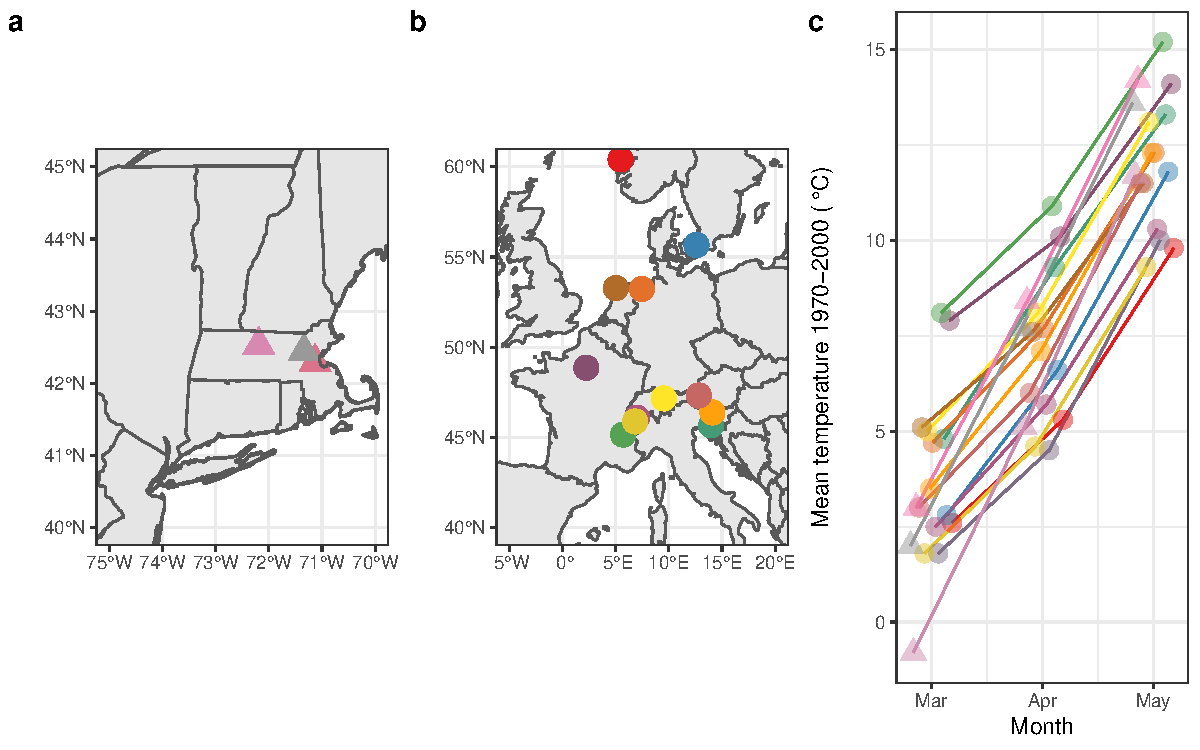
\includegraphics[width=1 \textwidth,trim=0cm 0cm 0cm 0cm, angle=0, scale=.9, origin=c,clip=false]{sampling_sites}
		\caption{Map of collection sites of (A) invasive populations in New England and (B) native populations in Europe and (C) average March, April, and May temperatures at each site. Note that spring temperature at native populations (circles) are comparable to spring temperature experienced by invasive populations (triangles)} 
		\label{fig:sites}
	\end{figure}


	\subsection{Experimental Design} 
	To test phenological responses to climate, seeds were exposed to eight treatments representing varying climates. Seeds were first subjected either a long or short stratification treatment, and then planted in one of four temperature treatments. All treatments were carried out in growth chambers. For each treatment, 20 representatives of each species (with seven invasive species this equals 140 seeds per treatment) and an additional five representatives of each local population of \textit{Plantago lanceolata} (the most heavily sampled species, with 13 populations) leading to a total of 205 seeds per treatment. Germination, time to germination, and aboveground linear height were recorded. Local population representatives were drawn from the greatest diversity of seed families, and seed family representation was equal across treatments. 
	
	\subsection{Stratification} 
	We stratified all seeds at 4$^\circ$C, 70\% humidity, 380 ppm of $CO_2$ \parencite[e.g.,][]{Meekins1999,Popay1970} on moistened Whatman 1 qualitative filter paper in sterile, vented, light-version Greiner bio-one 94x16 petri dishes in darkness \parencite{Baskin1998,Popay1970} in a single Biochambers TPC-19 Reach-In Growth Chamber for either 30 days or 60 days. These two stratification treatments represent intermediate stratification lengths for our species: studies show stratification of our species vary from 16 days \parencite{Popay1970} to 120 days \parencite{Meekins1999}. We began the 60-day stratification treatment in late September 2015; other seeds remained in paper envelopes at room temperature until they were in turn stratified in late October 2015.  Water was added to petri dishes every 30 days.
	
	\subsection{Germination}
	On November 23, 2015, seeds from both stratification treatments were transferred into individual pots with soil (see Experimental Design, above), which were placed into four different growth chambers (three Biochambers TPC-19 and one Biochambers LTCB-19 Reach-In Growth Chamber) and subjected to four different germination treatments. Temperature varied across treatments---all other measured variables were kept constant, and treatments were rotated through growth chambers to control for unmeasured chamber effects. (Seeds that germinated during stratification were not included in the analysis, but this was a small number and unlikely to affect results.)
	
	\paragraph{Germination Temperature:} Our four treatments used temperatures between 18 and 32$^\circ$C. Optimal weed germination typically occurs at 20-30$^\circ$C \parencite{Hartmann2010,Steinbauer1957,Wulff1994,Popay1970}. We used this  sightly broader spectrum to ensure a sufficient variance in germination response.
	
	\paragraph{Thermoperiocity:} Our treatments employed daily fluctuations in temperature---thermoperiocity---of 10$^\circ$C \parencite[see e.g.,][]{Steinbauer1957, Toole1963,ISTA1954}, translating to treatment temperatures of: 18/8$^\circ$C, 22.67/12.67$^\circ$C, 27.33/17.33$^\circ$C, and 32/22$^\circ$C. All treatments were subjected to 8 hours at the high temperature and the remaining 16 hours at the low temperature \parencite{Baskin1998,Roberts1981,Popay1970,Probert2000}. %About 80\% of weeds studied in \textcite{Steinbauer1957} and about 75\% of cultivated seeds germinate better with thermoperiocity (i.e., daily fluctuations in temperature)\parencite{Toole1963,ISTA1954}. 

	\paragraph{Light type:} We used T5HO fluorescent lights \parencite{Toole1963}, which have a high R:FR ratio as, generally, exposure to a high R:FR ratio increases germination rates \parencite[though some studies find germination requires high R:FR ratio or is insensitive,][]{Popay1970,Pons2000,Wulff1994}. % Germination rates typically increase when seeds are exposed to light \parencite[e.g.,][]{Baskin1998,Pons2000,Popay1970}. 
	
	\paragraph{Period/luminance of light:} We exposed all treatments to eight hours \parencite[coinciding with the higher temperature,][]{Baskin1998} of 75 micromol/m\textsuperscript{2}/second, which yielded a daily photon dosage of 2.16 mol/m\textsuperscript{2}. This amount of light should be sufficient to evoke germination response in all species \parencite{Pons1991}. Because none of our species are known to exhibit high-irradiance response, we erred on the side of too much light (see Supp. for additional details).
	
	\paragraph{Planting substrate:} We planted each seed in its own tray cell, on top of Fafard Growing Mix (a mixture of fine peat moss, fine perlite, and vermiculite) soil. We planted seeds on top of soil to ensure light availability \parencite{Tester1987} and because some species germinate poorly on filter paper \parencite{Andrews1974}.
	
	\paragraph{Water:} Every two days, seeds were watered until all of the soil had become wet \parencite{Steinbauer1957}; but not so much that a film of water covered the seeds \parencite{AOSA1960}.
	
	\paragraph{Germination and growth rate monitoring:}  Collection of germination and growth data was blind to population. Seeds were checked during the light period for germination every two days. Germination was defined as the growth of shoot or radical through the seed coat \parencite{Baskin1998,Popay1970}. Germination date for each seed was recorded.  Germination was monitored until 2016-01-29, for a total observation length of 67 days  \parencite[this is longer than the typical two-week germination trials according to][]{Baskin1998,Wulff1994}. Aboveground linear height of each seedling was measured five times: 2015-12-07, 2015-12-15, 2015-12-21, 2016-01-04, and 2016-01-29. Plant height was roughly linear with time (see Figure \ref{fig:lmgr}), so growth rate was defined as $\beta$ in the linear model: $height = \alpha + \beta*day + error $. This growth rate was calculated for each seed that germinated. On 2016-01-01, the plants were moved from the growth chambers to a greenhouse subject to the following conditions: natural photoperiod (approximately 10 hours of light/day), 20 to 25$^\circ$C, and 65\% humidity.
	\subsection{Statistical analysis} 
	Testing for evidence of rapid evolution in complex multi-species, multi-population designs can be challenging using classic frequentist approaches without balanced sampling and high replication. Thus we used a Bayesian multilevel modeling framework to enable fitting a model including full effects, and estimated variance, of species, population and seed family \parencite{Carpenter2017}. This yielded estimated (fixed) effects that transcend this variability in species, populations, and seed families to reveal generalized patterns. 

For all models (growth rate, germination rate, and germination timing), stratification length, continental origin, and temperature were treated as binary fixed effects, with the full suite of 2- and 3-way interactions included. Europe, 18/8$^\circ$C, and 30 days were reference levels for origin, temperature, and stratification length, respectively; temperature was recoded as three dummy binary factors, allowing non-linear responses to temperature. Seed family was treated as a random effect, nested within sampling population, nested within species (with random slopes and intercepts). Growth rate was modeled with a normal error distribution: 

\begin{align}
y_i =&  N(\mu_i,\sigma)\\
  \mu_i =&  \alpha_{sp[pop[sfamily[i]]]} + \beta 1_{sp[pop[sfamily[i]]]}\times origin +  \beta 2_{sp[pop[sfamily[i]]]} \times strat\\
          & +\beta 3_{sp[pop[sfamily[i]]]}\times temp1 +  \beta 4_{sp[pop[sfamily[i]]]}\times temp2 + \beta 5_{sp[pop[sfamily[i]]]}\times temp3 \notag \\
          & 
 		 + \beta 6_{sp[pop[sfamily[i]]]}\times origin\times strat  + \beta 7_{sp[pop[sfamily[i]]]}\times origin \times temp1 \notag\\ &
 		 + \beta 8_{sp[pop[sfamily[i]]]}\times origin \times temp2 + \beta 9_{sp[pop[sfamily[i]]]}\times origin \times temp3 \notag \\ &
 		 +\beta 10_{sp[pop[sfamily[i]]]}\times strat\times temp1 +\beta 11_{sp[pop[sfamily[i]]]}\times strat \times temp2 \notag \\ &
 		 + \beta 12_{sp[pop[sfamily[i]]]}\times strat \times temp3_ + \beta 13_{sp[pop[sfamily[i]]]}\times origin \times strat \times temp1 \notag\\ &
 		 +\beta 14_{sp[pop[sfamily[i]]]}\times origin \times strat \times temp2 + \beta 15_{sp[pop[sfamily[i]]]}\times origin \times strat \times temp3 )\notag
 \end{align}
 \begin{align}
 		 \intertext{Where the $\alpha$ and each $\beta$ coefficient were specified with nested random effects. For each $\gamma$ in $[\alpha,\beta 1:\beta 15]$:}
 		 \gamma_{sp[pop[sfamily[i]]]} =& N(\mu_{\gamma_{sp[pop[j]]}}, \sigma_{\gamma_{sp[pop[j]]}}) \\
 		 \gamma_{sp[pop[j]]} = & N(\mu_{\gamma_{sp[k]}}, \sigma_{\gamma_{sp[k]}}) \\
 		 \gamma_{sp[k]} = & N(\mu_{\gamma}, \sigma_{\gamma})
\end{align}


	 Where $sp = $ species, indexed with $k$, $pop =$ sampling population, indexed with $j$, $sfamily =$ seed family, indexed with $i$, and $strat$ = stratification. Germination rate was modeled similarly to growth rate, but using a binomial error distribution and logit link function, while germination timing was modeled with a Poisson error distribution and log link function. 
	 	
	All models were estimated using four chains, each with 2000 iterations (1000 devoted to warm-up), and wide priors. All models were built with Stan \parencite{Carpenter2017} using \texttt{rstanarm} version 2.17.4 \parencite{Goodrich2018} in R \parencite{Team2015}. Chain convergence was confirmed using the Gelman-Rubin statistic/$\hat{R}$ close to one \parencite{Gelman1992}. Model implementations were validated using simulated data; model fits were assessed using posterior predictive checks \parencite{Gelman2004}.  
	
	\paragraph{Average predictive comparisons:} The interactions of treatments (stratification and temperature) and random effects (species, population and seed family) make this model complex, and can make clear interpretations of parameter estimates difficult. To address this, we calculated average predictive comparisons \parencite{Gelman2007} for each stratification and  temperature level. These estimates average over interaction terms and the full mixed (fixed and random) effects, to provide a single estimate per level that includes all modelled uncertainty. Additionally, unlike model output from Poisson and Binomial models, which are given in transformed units, average predictive comparisons yield estimates that are in the units of the dependent variable (but always positive) \parencite{Gelman2007} and thus allow comparisons across effects. We note that average predictive comparisons can be complicated to implement in many unbalanced designs; because our stratification and temperature variables are balanced and independent (i.e., every combination of input values is equally likely to co-occur), we calculated average predictive comparison without any weighting requirement, thus simplifying the computation. 
	
	\paragraph{Data, code} 
	Data and R code is available on github at XXX
	\section{Results} 
	\paragraph{Germination rate:} Germination rate was high: 76\% of seeds germinated. Overall, germination rate was insensitive to temperature, stratification, or origin---95\% credible intervals (CrI) for all effects were clustered around zero (Figures \ref{fig:coef}, \ref{fig:rawrate}; Table \ref{tab:mod_rate}). Regardless of the climatic conditions, they germinated at fairly constant, high rates. Seeds from the invasive and native ranges germinated at similar rates and responded similarly to treatments. Seeds from different local populations also germinated at similar rates (see Figure \ref{fig:pops}).
 %(95\% CrI: round(invlogit(mod_rate$stan_summary[2,4]),2)--round(invlogit(mod_rate$stan_summary[2,10]),2))
	\paragraph{Germination timing:} The mean time to germination was 12.33 days.  Overall, all species germinated slower at the lowest temperature, but germinated at similar, faster speeds at the three higher temperatures, showing that temperature response is non-linear  (see Figures \ref{fig:coef}, \ref{fig:rawtime}; Table \ref{tab:mod_time}). Overall, stratification and seed origin had no noticeable effect; however, \textit{Plantago lanceolata} did show faster germination in response to med-low temperature $\times$ stratification interaction (see Figure \ref{fig:pops}).  Moreover, all species showed a significant positive interaction effect of origin, stratification and the higher temperature (95\% CrI: 1.05--2.9 days). 
	Populations showed fairly homogeneous responses, though temperature $\times$ stratification interactions did show some inter-population variability (see Figure \ref{fig:pops}). 
	\paragraph{Growth rate:} The mean growth rate was 1.2 mm/day. Overall, growth rate was the most sensitive to treatments, though it was still unaffected by stratification length or population origin (see Figures \ref{fig:coef}, \ref{fig:rawgrowth}; Table \ref{tab:mod_gr}). Growth rate decreased at warmer temperatures for all species, but especially \textit{Dactylis glomerata}. This effect was larger for each higher temperature; this is in contrast to germination timing, where the decrease with temperature was more constant (see comparison in absolute change displayed in Table \ref{tab:apc}). However, this decreased growth rate at high temperatures was not uniform across all treatments: for one of the higher temperatures (temp2) seeds stratified for 60 days and originating in North America (the invasive range) grew 0.74mm faster per day (95\% CrI: 0.22--1.27) than those stratified for 30 days from Europe (see `origin $\times$ strat $\times$ temp2' in Table \ref{tab:mod_gr}). 

% latex table generated in R 3.5.1 by xtable 1.8-3 package
% Mon Jan 20 11:15:45 2020
\begin{longtable}{rlll} 
\caption{Average predictive comparisons provide an additional interpretation of the results. They show, on average, how much change in the dependent variable results from a one unit change in the predictor variable. Note that all changes, whether positive or negative, are reported as positive. The table shows that higher temperatures had indistinguishable effects on germination timing, but sequentially bigger effects on growth rate.}
\label{tab:apc}\\
	\hline
	variable & germination rate (fraction) & germination date (days) & growth rate (mm/day) \\ 
	\hline
	stratification & 0.44 $\pm$ 0.02 & 9.6 $\pm$ 0.52 & 0.42 $\pm$ 0.02 \\ 
	temperature 1 & 0.39 $\pm$ 0.03 & 10.2 $\pm$ 0.34 & 0.29 $\pm$ 0.03 \\ 
	temperature 2 & 0.39 $\pm$ 0.03 & 10.2 $\pm$ 0.35 & 0.79 $\pm$ 0.03 \\ 
	temperature 3 & 0.38 $\pm$ 0.03 & 10.3 $\pm$ 0.34 & 0.91 $\pm$ 0.03 \\ 
	\hline\\
	\hline
\end{longtable}

\begin{sidewaysfigure}
	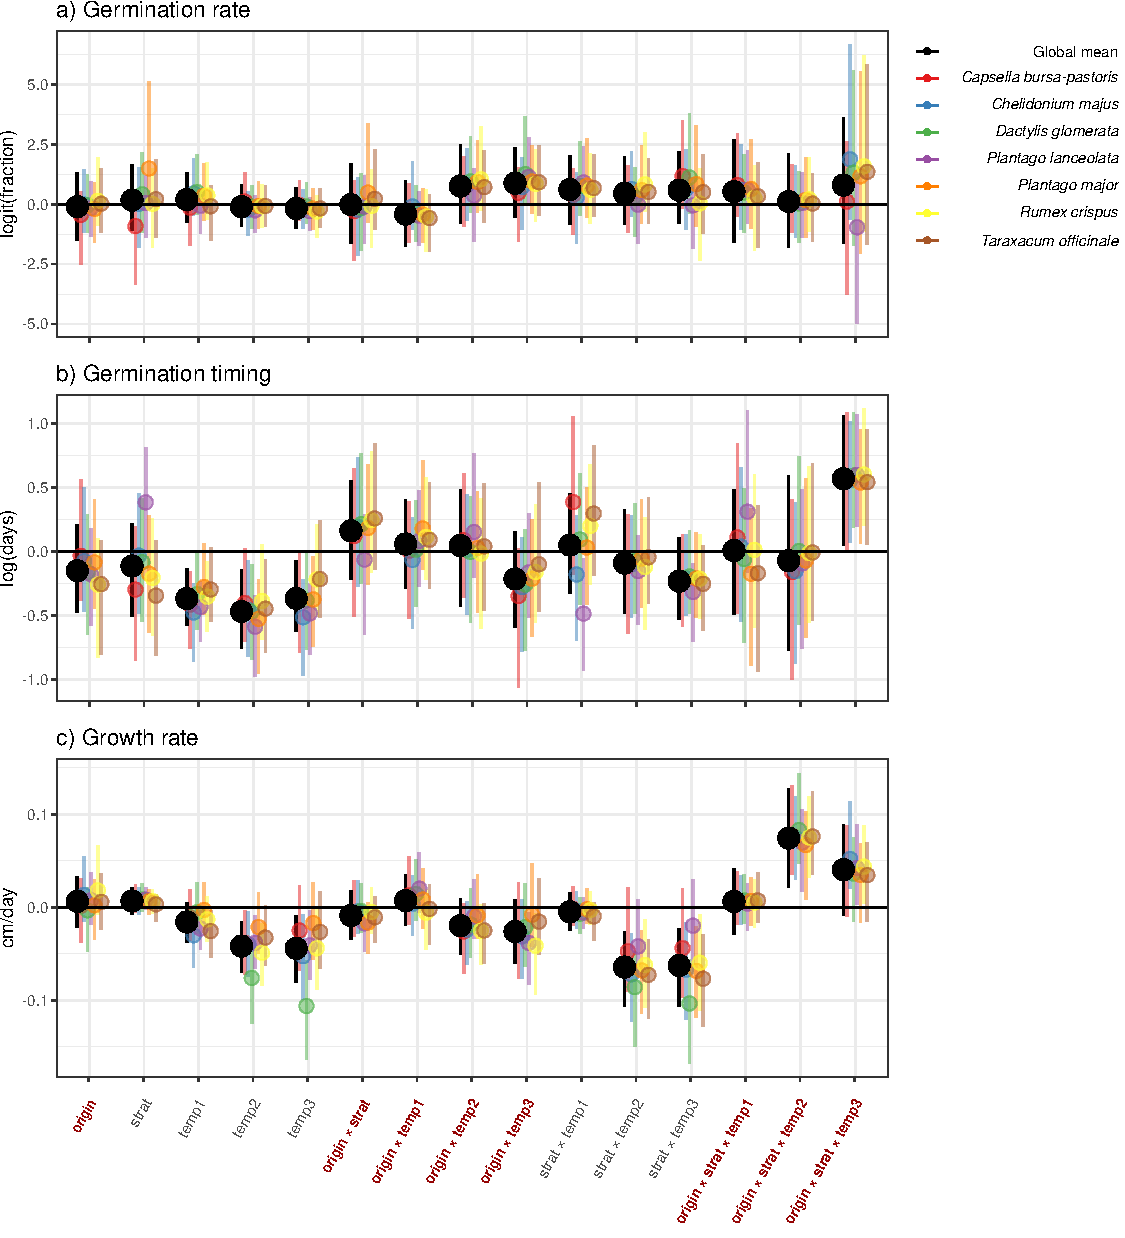
\includegraphics[width=1.1\textheight, scale=.7]{germ_figs_onepage.pdf}
	\caption{Multilevel model coefficients with 95\% credible intervals, showing global average effects and species random effects. Intercept coefficients provided in the Supp. in Tables \ref{tab:mod_rate},\ref{tab:mod_time}, \ref{tab:mod_gr}.  a) model of germination rate, b) model of germination timing and c) model of growth rate.}
	\label{fig:coef}

\end{sidewaysfigure}

	\section{Discussion}
	
	This study leveraged the power of a multi-species growth chamber experiment of native and introduced populations to investigate the importance of rapid evolution for invasive species' success. Across seven highly invasive plant species, we found only isolated support for the prevalence of post-introduction rapid evolution of key invasion traits---germination rate, timing, and growth rate. Instead, our results support the theory that these traits do not need to evolve for these species to invade: weediness, wide environmental tolerance, plasticity, or generalist traits in the source populations likely provide sufficient capacity to exploit novel environments \parencite{Baker1965}. Rapid evolution may provide a helping hand, but---at least for these traits and these species---rapid evolution does not appear essential for invasion success.
	
	These findings are especially pronounced in germination rate, where all species germinated well and with scant sensitivity to climatic conditions, suggesting that the source populations of invading species provided invaders with the capacity to germinate in diverse environments, without evolving. Some have suggested that while initially species may not need to evolve, they may once achieving a foot-hold \parencite{Lamarque2015}. However, many of the study species (e.g., \textit{Dactylis glomerata}) have occupied their invasive range for centuries, yet still show little sign of an evolving, or evolved, germination response. 
	
	Overall, germination timing and growth rate did not show signs of post-invasion evolution. However, there was some evidence that particular responses have evolved: North American (invasive) populations germinate later and grow faster under high-temperature/long stratification combinations. Taking the climate of North American populations into account (Figure \ref{fig:sites}), this growth rate evolution may be adaptive. North American populations experience climates with longer winter stratification  (lower mean March temperatures) and hotter growing temperatures (higher mean May temperature). Thus, the capacity to grow faster at high temperatures after being exposed to our long stratification treatment may provide fitness advantages. Although it is  possible that these differences could be residual founder effects \parencite{Shirk2014}, a result of genetic drift \parencite{Eckert1996}, or that germination rate is not a fitness trait,  the convergence with experienced climate suggests that this observed change in growth rate is a sign of adaptive evolution. 
	
	These results highlight the need to condition biological invasion mechanisms on specific invasion traits. We found that rapid evolution played no role in germination rate, but did play a limited role in growth rate for these species. This suggests that research and theory aimed at identifying which traits are likely to rapidly evolve with invasion may yield more insights than testing for an overall mechanism of invasion that is consistent across traits. We found evidence that germination timing and growth rate traits were most likely to evolve in response to specific combinations of spring temperatures and winter length. This result suggests that considering the interdependent multivariate environment in the invasive range may be critical for predicting how traits evolve post-introduction. 
%	Furthermore, the types of environmental variables in which these traits evolve in response to can also be illuminating. Our results suggest that traits are most likely to evolve in response to specific combinations of spring temperature and winter length.  Adaptation to winter length is especially under-studied, and our results suggest that examining it is most useful in concert with other climate variables.  
Not only can these trait evolution/environment relationships be useful for understanding invasions, they can also help delineate plant capacities to adapt to the multifaceted effects of anthropogenic climate change. 
	
	Our findings preliminarily suggest that these invasive species may be able to adapt to changing climates. Because cold-stratification is a simulation of temperate winter, the evidence that species can adapt their growth rate in accordance with winter length and spring temperature suggests that they may have the capacity to adapt to changing winter lengths and spring temperatures that anthropogenic climate change is bringing \parencite{IPCC2015}. These results also echo the  importance of varying both winter length and spring temperature in order to observe responses to climate change \parencite[e.g.,][]{Bernareggi2016}. 

	Our results come from a limited number of individuals and populations collected from the invasive range (see Figure \ref{fig:sites}; Table \ref{tab:seeds}), yet our sampling sites show substantial climate variation (Figure \ref{fig:sites}), highlighting potentially important climatic differences between Europe and North America that may shape invasions. While additional sampling across the invasive range would have yielded greater geographical inference to our findings, it may also have made the complex stratification by temperature responses harder to detect---if such responses are specific to local climate regimes. Based on our findings, we suggest sampling across distinct invasive range climates could help understand which traits evolve where post-introduction. Such studies could leverage Bayesian modeling to include climate as a predictor, while controlling for other factors. 

	Our study leveraged the benefits of growth chambers to provide a common set of precisely controlled multivariate environments for seven species; however, the benefits of this design  trade off with a lack of realism. Reciprocal field common garden experiments can integrate important factors, such as biotic interactions, which may be important for determining invasions \parencite{Germain2018,Blois2013}. Yet by focusing on multivariate climate and controlling for all other factors, we were able determine that rapid evolution appears largely unimportant for invasion success in a range of introduced climates. Furthermore, while common garden experiments are fundamentally idiosyncratic and resource-intensive, our growth chamber design and Bayesian modeling approach could be seamlessly harnessed by other research teams to test other invasive species, other populations, other traits, and other combinations of climate factors (including precipitation). Such future small-scale growth chamber studies could enable robust meta-analyses capable of identifying the traits and climate responses for which rapid evolution is, or is not, essential for invasion success. 
	
	Our results show that rapid evolution of germination and growth traits is unlikely to be essential for all invasion success. Instead, it seems that broad environmental tolerance is key to invasion success for these seven species. Rapid evolution may still play a role, especially in more extreme or different environments:  \textcite{Linde2001} found that \textit{Capsella bursa-pastoris} evolved to colonize high-altitude and desert environments in California. However, we found little sign of evolution in our comparisons between temperate populations of this species. Perhaps, as suggested by \textcite{Baker1965}, the generalist traits contained in temperate source populations are suitable as long as the introduced environment is not too different. Our findings provide support for  the speculation by van Kleunen and colleagues (2010) that future invasions can be predicted by species' characteristics, but perhaps only specific traits, such as germination rate. This finding suggests that managers can perhaps best guard against future invasions by targeting weedy species and preventing them from dispersing beyond their native ranges. 
\section{Acknowledgments}
This field work was supported by the Harvard College Research Fund and the Harvard University Center for the Environment Undergraduate Summer Research Fund. Thanks to E. Forrestel for mentorship to HNE. Thanks to J. Williams and H. Branch for fruitful discussions. Thanks also to D. Flynn, S. Gee, J. Samaha, and T. Savas for help transplanting, collecting, and measuring. Thanks to F. Rosin, K. Woodruff, and J. Gard for help with collection and growing logistics. Thanks to S. Fritz for help with data input. Thank you to M. Rucinski, C. Husic, N. Gilbert, A. Delgado, and A. Acosta for comments on earlier drafts of this paper. Thanks to J. Eyster, S. Stalhandske, and G. Barbone for assistance with and camaraderie during field sampling. 

	

\section{Literature Cited}
\printbibliography
\end{document}
